% You should title the file with a .tex extension (hw1.tex, for example)
\documentclass[a4paper, 11pt]{article}
\usepackage{fancyvrb}
\usepackage{verbatim}
\usepackage{amsmath}
\usepackage{amssymb}
\usepackage{fancyhdr}
\usepackage{graphicx}

\usepackage[margin=1in]{geometry}
\usepackage{tikz}
\usetikzlibrary{automata,positioning,arrows}

\usepackage[margin=1in]{geometry}
\usepackage{listings}
\usepackage{color}

\definecolor{dkgreen}{rgb}{0,0.6,0}
\definecolor{gray}{rgb}{0.5,0.5,0.5}
\definecolor{mauve}{rgb}{0.58,0,0.82}

\lstset{frame=tb,
	language=Java,
	aboveskip=3mm,
	belowskip=3mm,
	showstringspaces=false,
	columns=flexible,
	basicstyle={\small\ttfamily},
	numbers=none,
	numberstyle=\tiny\color{gray},
	keywordstyle=\color{blue},
	commentstyle=\color{dkgreen},
	stringstyle=\color{mauve},
	breaklines=true,
	breakatwhitespace=true,
	tabsize=3
}

\newcommand{\question}[2] {\vspace{.25in} \hrule\vspace{0.5em}
	\noindent{\bf #1: #2} \vspace{0.5em}
	\hrule \vspace{.10in}}
\renewcommand{\part}[1] {\vspace{.10in} {\bf (#1)}}

\newcommand{\myname}{Possawat Sanorkam}
\newcommand{\myemail}{possawat2017@hotmail.com}
\newcommand{\myhwnum}{2}

\setlength{\parindent}{0pt}
\setlength{\parskip}{5pt plus 1pt}

\pagestyle{fancyplain}
\lhead{\fancyplain{}{\textbf{HW\myhwnum}}}      % Note the different brackets!
\rhead{\fancyplain{}{\myname\\ \myemail}}
\chead{\fancyplain{}{ICCS310}}

\begin{document}
	
	\medskip                        % Skip a "medium" amount of space
	% (latex determines what medium is)
	% Also try: \bigskip, \littleskip
	
	\thispagestyle{plain}
	\begin{center}                  % Center the following lines
		{\Large ICCS310: Assignment \myhwnum} \\
		\myname \\
		\myemail \\
		\today \\
	\end{center}
	
	\question{1}{Regex to NFA/DFA} %don't delete yet:(}
	
	\part{1} $a(abb)^* + b $
	
	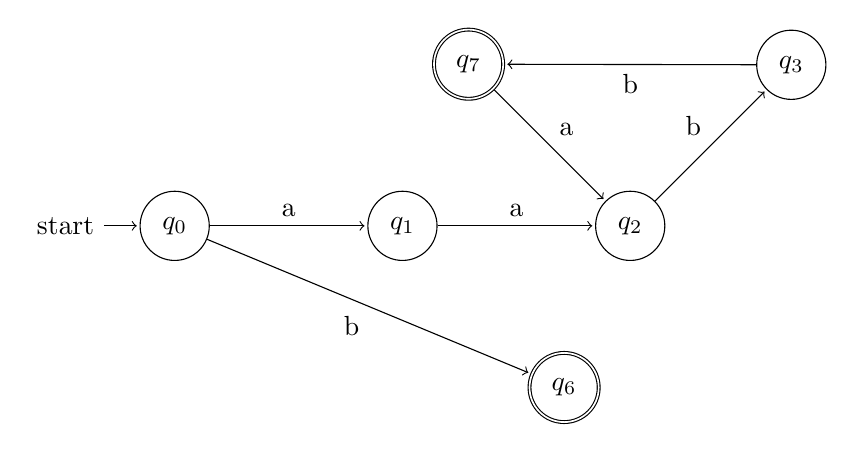
\begin{tikzpicture}[shorten >=1pt,node distance=2cm,auto] 
	\node[state,initial] (q_0)   {$q_0$}; 
	\node[state] (q_1) [ right=of q_0] {$q_1$}; 
	\node[state] (q_2) [ right=of q_1] {$q_2$}; 
	\node[state] (q_3) [above right=of q_2] {$q_3$}; 
	\node[state,accepting](q_6) [below right=of q_1] {$q_6$};	
	\node[state,accepting](q_7) [above left=of q_2] {$q_7$};
	\path[->] 
	(q_0) edge  node {a} (q_1)
	edge [swap] node {b} (q_6)
	(q_1) edge  node {a} (q_2)
	(q_2) edge  node {b} (q_3)
	(q_3) edge  node {b} (q_7)
	(q_7) edge  node {a} (q_2);

	\end{tikzpicture}
	
	\part{2} $(a + b)^* aa(a + b)^*$
	
	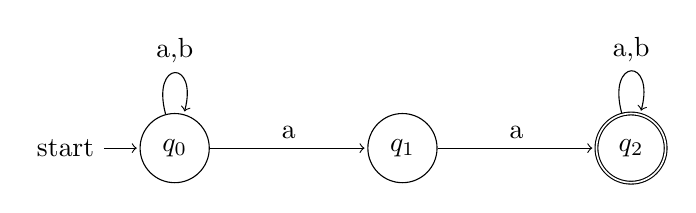
\begin{tikzpicture}[shorten >=1pt,node distance=2cm,auto] 
	\node[state,initial] (q_0)   {$q_0$}; 
	\node[state] (q_1) [right=of q_0] {$q_1$}; 
	\node[state,accepting](q_2) [right=of q_1] {$q_2$};
	\path[->] 
	(q_0) edge [loop above] node {a,b} ()
	edge  node {a} (q_1)
	(q_1) edge node {a} (q_2)
	(q_2) edge [loop above] node {a,b} ();
	\end{tikzpicture}

	\part{3} $a^+ + (ab)^+$
	
	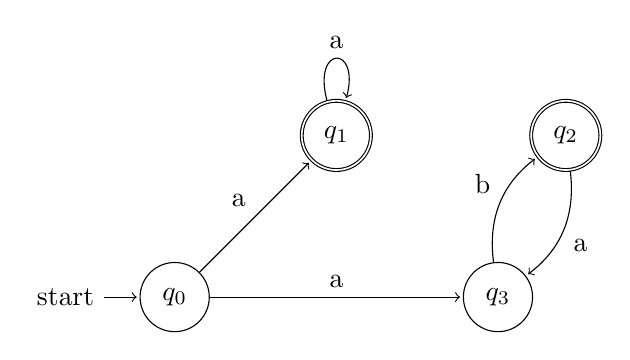
\begin{tikzpicture}[shorten >=1pt,node distance=2cm,auto] 
	\node[state,initial] (q_0)   {$q_0$}; 
	\node[state,accepting] (q_1) [above right=of q_0] {$q_1$}; 
	\node[state,accepting](q_2) [right=of q_1] {$q_2$};
	\node[state] (q_3) [below right=of q_1] {$q_3$}; 
	\path[->] 
	(q_0) edge  node {a} (q_1)
	edge node {a} (q_3)
	(q_1) edge [loop above] node {a} ()
	(q_2) edge [bend left]  node {a} (q_3)
	(q_3) edge [bend left]  node {b} (q_2);
	\end{tikzpicture}
	
	\question{2}{Finite-State Machines to Regex}
	
	\part{1} $ \varnothing^* $ (Rejecting any input)
	
	\part{2} $a^* + a^*b^+a^+b$ (Contains only $a$s or any pattern of $a$s to $b$s to $a$s to $b$s.)\\\\\\\\
	
	\question{3}{Binary Addition}
	
	$$A = \{w \in \Sigma^* \text{ $|$ } \text{ the bottom row of w is the sum of the top two rows } xy \in L_1 \}$$
	
	Prove that A is regular.
	
	{\em Proof}: Since, $A$ only accept column vectors of size 3 such that the bottom row of w is the sum of the top two rows, it is difficult create a machine that recognize $A$ directly. We know that binary addition start by summing the least significant bits, including transferring a carry when the bit overflow. So, reading the string in reverse will be simpler since we can transfer the carry from the last column to the next column on the left directly. 
	
	From the lemma, if $L$ is a regular language, then $L^R$ is also regular. We want to show that $A^R$ is a regular language. Let $L(M) = A^R$. So, $M$ is a machine that recognize $A^R$, else we can call it the binary adder.
	
	$M$ is machine that translate each vector into transfer bit and send it to the next state. It only accepts the string that follow its calculation (The sum of first row, second row and carry bit must be equal to the third row). If both numbers are 1 on first and second rows, we send it the the state which refers to a carried bit included state. There are 2 states, $q_1,\text{and }q_2$.
	
	$q_1$ is the accepting state with no carry bit transferred.
	
	$q_2$ is the state with carry bit. (Not done with the addition yet)
	
	We can mathematically define a function of LSB addition as $a \odot b = c$ and a function of carry bit as $carry(x,y,z)$. The transition of this machine follows that $x_1 \odot x_2 + \text{ carry bit state } = x_3$ must be satisfied and the next transition depends on the carry bit from $carry(x_1, x_2, \text{ carry bit state }) $ whether it will be $q_1 or q_2$. Hence, $A^R$ is regular and that makes $A$ regular also from the lemma.
	
	Therefore, A is regular. $\square$
	
	\question{4}{Division Operation?} 
	
	$$\frac{L_1}{L_2} = \{x \text{ $|$ } \exists \in L_2 \text{ s.t. } xy \in L_1 \}$$
	Prove that if $L_1$ and $L_2$ are regular, then $\frac{L_1}{L_2}$ is also regular.
	
	{\em Proof}: 
	From a lemma, for every regular expression $R$, there is a DFA that recognizes the language $L(R)$.
	Suppose $L_1$ and $L_2$ are regular, then there exist DFA $M_1 =(Q,\Sigma,\delta,q_0,F_1)$ which accepts $L_1$ and DFA $M_2 =(Q,\Sigma,\delta,q_0,F_2)$ which accepts $L_2$. We want to show that $L_3 = \frac{L_1}{L_2}$ where $L_1, L_2, L_3 \in \mathbb{I}$.
	
	We have that $Q, \Sigma, \delta, \text{and } q_0$ in $M_1$ and $M_2$ can be shared, just that the accepting states are different. $L_3$ then can be recognized by some DFA $M_3 = (Q,\Sigma,\delta,q_0,F_3)$. We know that $\Sigma$ is a number digit alphabet (0-9). Then, each state is just an integer. So, $\forall x \in F_1, \exists y \in F_2, \text{and } \exists z \in F_3, zy = x$.
	
	From the observation, $L_1$, which is regular, contains accepting states that made of $zy$ from $F_2$ and $F_3$. Also, $L_2$, which is regular, recognized by $M_2$ and we can choose any number to be an accepting state in $F_2$ (As long as we accept at least a number). Since $F_3$ can be any state (number) also, there always exist $z$ that will satisfied $zy = x$. Thus, $M_3$ exists since we can design $F_3$. %I guess?
	
	Therefore, if $L_1$ and $L_2$ are regular, then $\frac{L_1}{L_2}$ is also regular. $\square$
	
	\question{5}{Does It Accept Everything?}
	Let $M = (Q, \Sigma, \delta, q_0, F)$.
	
	{\em Solution}: Every finite-state machine is simply a directed graph, then we can check it by performing this algorithm.
	
	Let $strs = \Sigma^*$, given size of $\Sigma$ is a constant. Also, $E$ = edges that we can refer to $\delta$.
	
	First, we design a function called $is\_recognize$ that check if a string can be recognized from $M$ by forming a directed graph using $M$, which is the given machine, then perform a traversal to get the final state (cycles are ignored since we stopped on the last character). This would take $O(|Q|+|E|)$ to create the graph. Suppose we have infinite amount of memory, then we can store this graph to use later. If any string rejected, then we set the $accept$ to false, which means machine M rejects $\Sigma^*$. Hence, assuming amortized running time for getting an item from a hash set is $O(1)$, then the time complexity would be $O(str)+O(1)+O(1) = O(str)$.
	
	Second, we make sure that we can enumerate through $strs$. If we have infinite power of computation, we can perform $is\_recognize$ on each string in $strs$ at the same time. Then, the time complexity would be $O(str)$. If not, we can iterate on each string instead, which will definitely take longer time. Let $ns =$ number of strings in $strs$, it would take $O(str*{ns})$.
	
	Finally, return whether we accept it or not. Total time complexity $O(|Q|+|E|+str)$ in parallel or else $O(|Q|+|E|+str*{ns})$.
	\\\\\\
	The pseudo-code is given below.
	
\begin{Verbatim}[numbers=left]
//global variables
G = create_graph(M) //a graph using Q as vertices and E from DFA
accept = true //assume that this variable is thread-safe globally
is_recognize(str){
	count = 0 //First character
	n = length of str - 1
	current_state = str[count]
	while(count < n){
		next_char = str[count+1]
		
		//using map of edges of current_state to go to next state
		current_state = go_next(current_state,next_char)
		count++ //increment count
	}
	if(current_state not in F){
		accept = false 
		//if there is any rejection, reject it globally.
	}
}

accept_all(strs){
	//parallel mapping is_recognize on every string
	strs.par_map(is_recognize)
	return accept
}
\end{Verbatim}

%I tried to make one that runs in polynomial time in |Q| assuming the size of Σ is constant, but it is so difficult.
	
	
	\question{6}{All The Same?}
	Multiplication and power simply make them equivalent like $2*4 = 4*2 === 2^4 = 4^2$.
	
\end{document}